\documentclass[a4paper]{tufte-handout}

\title{1. Introduction to FMO Theory \thanks{Wayne~W.~Z. Yeo}}

\author[MIT 5.60]{\textsc{Chem 215} Advanced Organic Chemistry \thanks{Course Instructor: David A. Evans}}

%\date{28 March 2010} % without \date command, current date is supplied

%\geometry{showframe} % display margins for debugging page layout

\usepackage{graphicx} % allow embedded images
  \setkeys{Gin}{width=\linewidth,totalheight=\textheight,keepaspectratio}
  \graphicspath{{graphics}} % set of paths to search for images
\usepackage{epstopdf}
\usepackage{amsmath,amsthm}  % extended mathematics
\usepackage{physics,siunitx}
\usepackage[version=4]{mhchem} \usepackage{chemmacros}
\usepackage{booktabs} % book-quality tables
\usepackage{units}    % non-stacked fractions and better unit spacing
\usepackage{multicol} % multiple column layout facilities
\usepackage{lipsum}   % filler text
\usepackage{fancyvrb} % extended verbatim environments
  \fvset{fontsize=\normalsize}% default font size for fancy-verbatim environments

% Standardize command font styles and environments
\newcommand{\doccmd}[1]{\texttt{\textbackslash#1}}% command name -- adds backslash automatically
\newcommand{\docopt}[1]{\ensuremath{\langle}\textrm{\textit{#1}}\ensuremath{\rangle}}% optional command argument
\newcommand{\docarg}[1]{\textrm{\textit{#1}}}% (required) command argument
\newcommand{\docenv}[1]{\textsf{#1}}% environment name
\newcommand{\docpkg}[1]{\texttt{#1}}% package name
\newcommand{\doccls}[1]{\texttt{#1}}% document class name
\newcommand{\docclsopt}[1]{\texttt{#1}}% document class option name
\newenvironment{docspec}{\begin{quote}\noindent}{\end{quote}}% command specification environment

\newtheorem{theorem}{Theorem}
\newtheorem{corollary}{Corollary}
\newtheorem{definition}{Definition}
\newenvironment{justification} {\begin{proof}[Justification]} {\end{proof}}

\begin{document}

\maketitle % this prints the handout title, author, and date

\begin{abstract}
\noindent
General bonding considerations. The \ce{H2} molecule revisited. Donor and acceptor properties of bonding/antibonding states. Hybridisation and electronegativity. Hyperconjugation.
\end{abstract}

%\printclassoptions

\section*{Universal effects governing chemical reactions}

\subsection*{1. Steric effects}

Non-bonding interactions between substituents within a molecule or between reacting molecules. These
are the closed-shell repulsion of occupied molecular orbitals of the reactants (\ce{4e-} filled-filled interactions).

\begin{equation}
  \Delta E_{\textrm{sterics}} = - \sum_{a,b} (q_a + q_b) \beta_{ab} S_{ab}
\end{equation}

\subsection*{2. Electronic effects}

The effect of through-bond and through-space polarisation by heteroatom substituents on reaction rates and selectivities.
This is the Coulombic attraction or repulsion between atoms of the reactants (ionic contribution).

\begin{equation}
  \Delta E_{\textrm{electronics}} = \sum_{k < l} \frac{Q_k Q_l}{\epsilon R_{kl}}
\end{equation}

\subsection*{3. Stereolectronic effects}

Geometric constraints placed upon ground and transition states by orbital overlap considerations.

\begin{definition}[Fukui Postulate]
  During the course of chemical reactions, the interaction of the highest filled (HOMO) and lowest unfilled (LUMO)
  molecular orbital in reacting species is preeminently important to the stabilisation of molecular structure.
\end{definition}

\section{Hyperconjugation: Stabilising Carbocations}

\begin{definition}[Stereoelectronic requirement for hyperconjugation]
There must be a \textbf{syn-planar} orientation between interacting orbitals.  
\end{definition}

\subsection{Physical evidence for hyperconjugation}

Bonds participating in the hyperconjugative interaction \ce{C-R} will be lengthened (as they are destabilised) while
the \ce{C-C+} bond is shortened.

\section*{Case Study: Endiandric Acids A and B}
\textbf{Paragraph 1.} A rather exciting introduction to a natural product paper. The key unique feature about these natural products is their occurrence as \textit{racemic} mixtures, despite the presence of
\textbf{eight} asymmetric centres. This is an unusual observation for naturally occurring compounds. How does nature
access both enantiomers? \marginnote{It's hard to imagine an enzyme being able to access a racemate without starting from an achiral pool.}

The courageous proposition by {\small \textsc{Black}} for the "biogenesis" of this family of compounds from achiral precursors, 
is a series of \textit{non-enzymatic} electrocyclisations governed by the \textbf{Woodward-Hoffmann} rules; making\marginnote{$8 \pi$ and $6 \pi$ \ce{e-} electrocyclisations are thermally-allowed.} this work 
particularly instructive for students of synthetic organic chemistry. The authors present two routes to the target: firstly, a stepwise, stereocontrolled synthesis \cite{nicolaou1982endiandricA}
and secondly, a biomimetic approach which experimentally verifies the non-enzymatic electrocyclisation hypothesis.

\subsection{Stepwise synthesis}

\textbf{Paragraph 2.} The authors describe a key bicyclic intermediate \textbf{7} resulting from a Wittig-type reaction

\subsection{Electrocyclic synthesis}

In 1980, it was proposed that $\mathbf{1}$ was formed from carboxylic acids by a series of thermally-allowed cyclisations allowed by Woodward-Hoffmann 
rules.\cite{nicolaou1982endiandricB} Firstly, an 8$\pi$ \ce{e-}
conrotatory electrocyclisation, followed by a 6$\pi$ \ce{e-}disrotatory electrocyclisation, and finally, an intramolecular [4+2]
cycloaddition (intramolecular \textbf{Diels-Alder}).

\pagebreak

\section*{What is Organic Synthesis?}

\begin{definition}[Transform]
  An imaginary retrosynthetic operation transforming a target molecule into a precursor molecule in a manner 
  such that bonds can be reformed or cleaved by known or reasonable synthetic, forward reactions.
\end{definition}

\subsection*{Retrons -- keying structural motifs to reactions}

\begin{definition}[Retron]
  The \textbf{minimal} substructural element in a target structure which keys the direct application of a \textbf{transform} to generate a synthetic precursor.
  This is a structural unit that signals the application of a particular strategy algorithm during retrosynthetic analysis.
\end{definition}

Recognising relationships between retrons and transforms is crucial to synthesis design. For example, a 1,3-dicarbonyl 
is a retron for the \textbf{Claisen condensation}.

A \textbf{full retron} is. Consequently, a \textbf{partial retron} is.

Full retrons are specific to particular reactions, reflecting \textit{exact} structural
requirements. In sharp contrast, partial retrons offer more flexibility
as they might be intermediates for several different full retrons and 
forward reactions.

\begin{definition}[Functional Group Interconversion]
  
\end{definition}

\section*{Diels-Alder Reaction}

The Diels-Alder reaction is the quintessential thermally-allowed $[4+2]$ cycloaddition.

\begin{marginfigure}%
  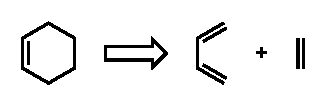
\includegraphics[width=\linewidth]{diels-alder-transform}
  \caption{Diels-Alder transform. Shown here is the simplest Diels-Alder reaction: the formation of cyclohexene from 1,3-butadiene and ethylene.}
  \label{fig:marginfig}
\end{marginfigure}

\section*{$[2+2]$ Photocycloaddition}

\bibliography{lec1}
\bibliographystyle{plainnat}

\end{document}